% !TeX program = pdflatex
% Optional rebuild: compile this file, then copy figure_plates.pdf into figures/.
% Custom large-format plates: 420 x 385 mm. No external fonts or shell escape.
\documentclass[10pt]{article}
\usepackage[T1]{fontenc}
\usepackage[utf8]{inputenc}
\usepackage[paperwidth=420mm,paperheight=385mm,margin=9mm]{geometry}
\usepackage{newtxtext,graphicx,xcolor,caption,microtype,tabularx}
\definecolor{forestink}{HTML}{186D30}
\definecolor{sourceblue}{HTML}{006786}
\definecolor{papergray}{HTML}{F3F2F2}
\pagestyle{empty}
\setlength{\parindent}{0pt}
\captionsetup{font=small,labelfont=bf,skip=4pt,justification=justified,singlelinecheck=false}
\begin{document}
{\large\bfseries\color{sourceblue} WORLDWIDE REPORTED ACCOUNT}\hfill {2025 reference estimates}\par
\vspace{2mm}\hrule\vspace{1mm}
\begin{center}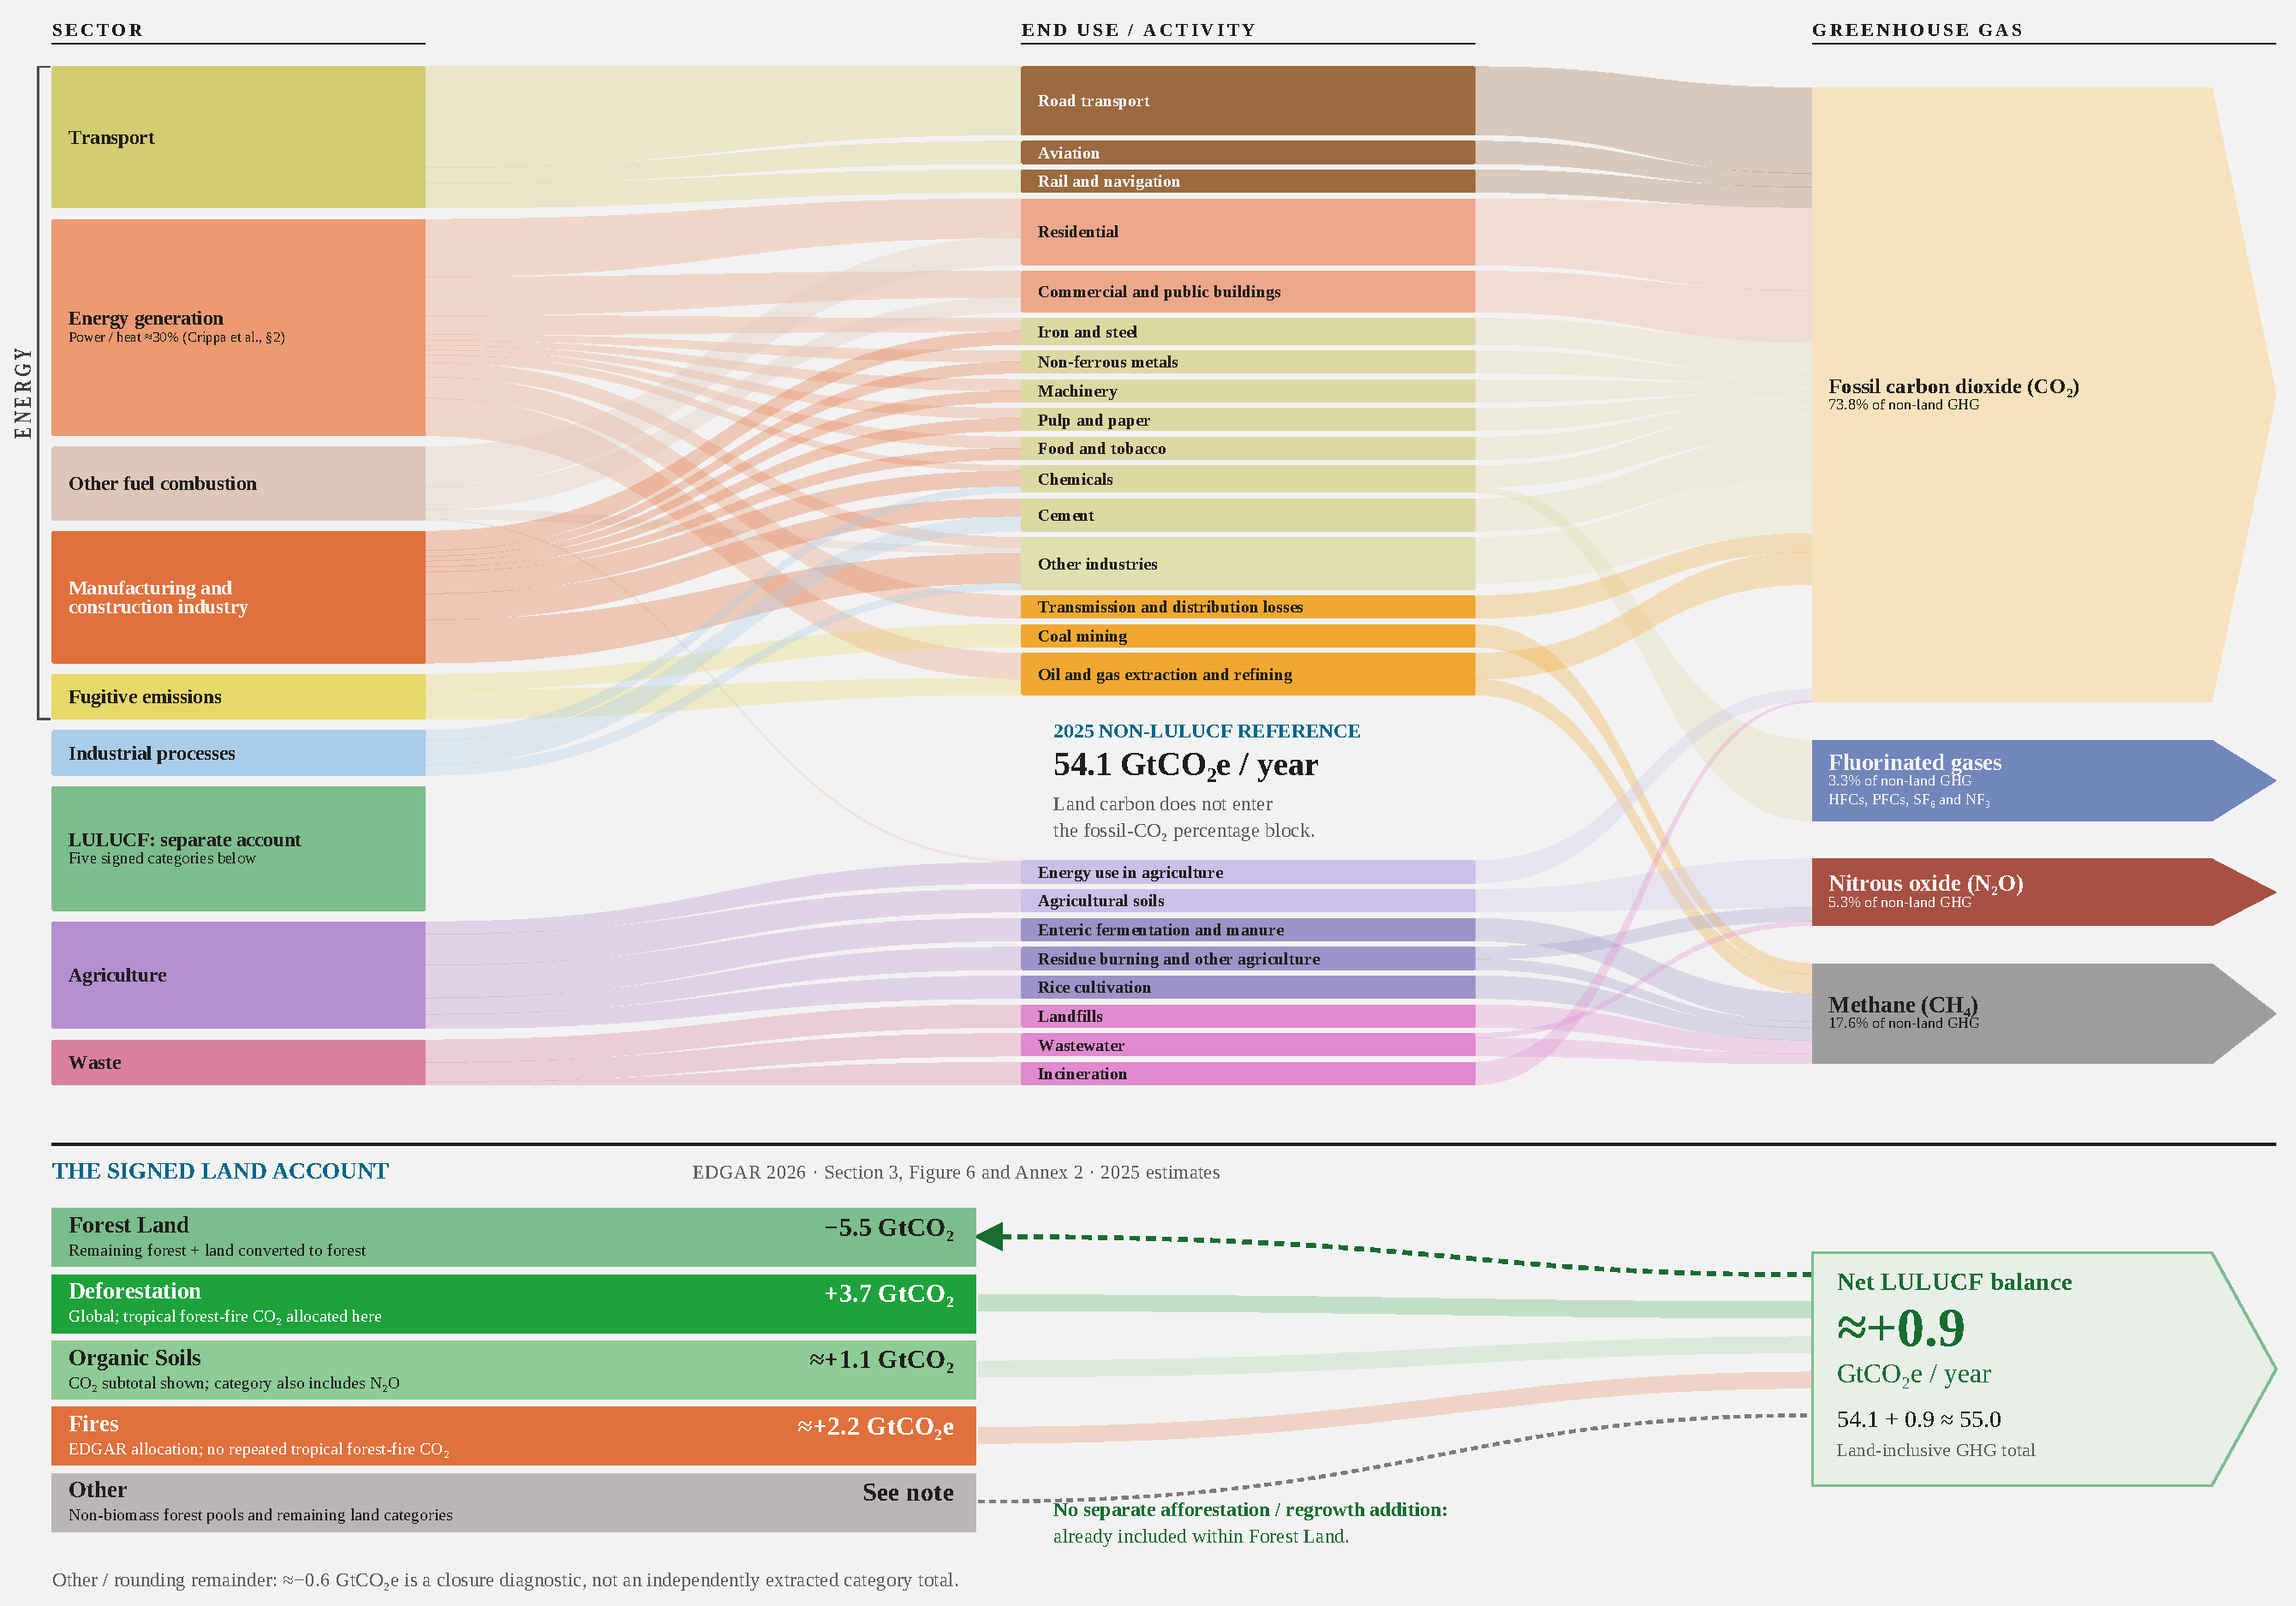
\includegraphics[width=385mm]{figures/figure1.pdf}\end{center}
\vspace{-3mm}
\fcolorbox{forestink}{papergray}{\parbox{.975\textwidth}{\vspace{1mm}
\textbf{Disjoint land categories, separate gas denominator.} Forest Land already includes land converted to forest; no extra afforestation or regrowth subtotal is added. Deforestation includes tropical forest-fire CO$_2$, which is excluded from Fires; tropical fire non-CO$_2$ gases remain in Fires. Organic Soils' quoted 1.1 is CO$_2$ only. The diagnostic remainder $0.9-[3.7-5.5+2.2+1.1]\simeq-0.6$ also absorbs omitted subcomponents and rounding; it is not a separately extracted Other estimate. Source: Crippa et al. (2026), booklet Sections 2--3 and Annex 2, doi:10.2760/7717504 (CC BY 4.0).\vspace{1mm}}}\par
\vspace{3mm}
\begin{minipage}{\textwidth}
\captionof{figure}{\textbf{The reported 2025 account and its boundaries.} The sector--activity--gas organization is adapted from WRI (2005) and Ecofys (2013), with author-created vector artwork and a separate five-category signed land account. Intermediate activity nodes describe pathways, rather than EDGAR's official sector list. Gas shares refer only to EDGAR's 54.1 GtCO$_2$e non-LULUCF inventory using AR5 GWP$_{100}$; 73.8\% is fossil CO$_2$. Land emissions therefore do not enter that gas block. The reverse dashed link denotes Forest Land's net removal. Forest/deforestation estimates use a global Tier 1 approach with default parameters and estimated activity data beyond the latest input maps, not independently remeasured 2025 carbon densities. Paths and all graphical areas are schematic, not a balanced quantitative Sankey. Electricity-attribution paths must not be counted again as direct emissions.}
\end{minipage}
\clearpage
{\large\bfseries\color{sourceblue} PANTROPICAL CARBON WITHIN A WORLDWIDE ACCOUNT}\hfill {Stock and annual transfer}\par
\vspace{2mm}\hrule\vspace{1mm}
\begin{center}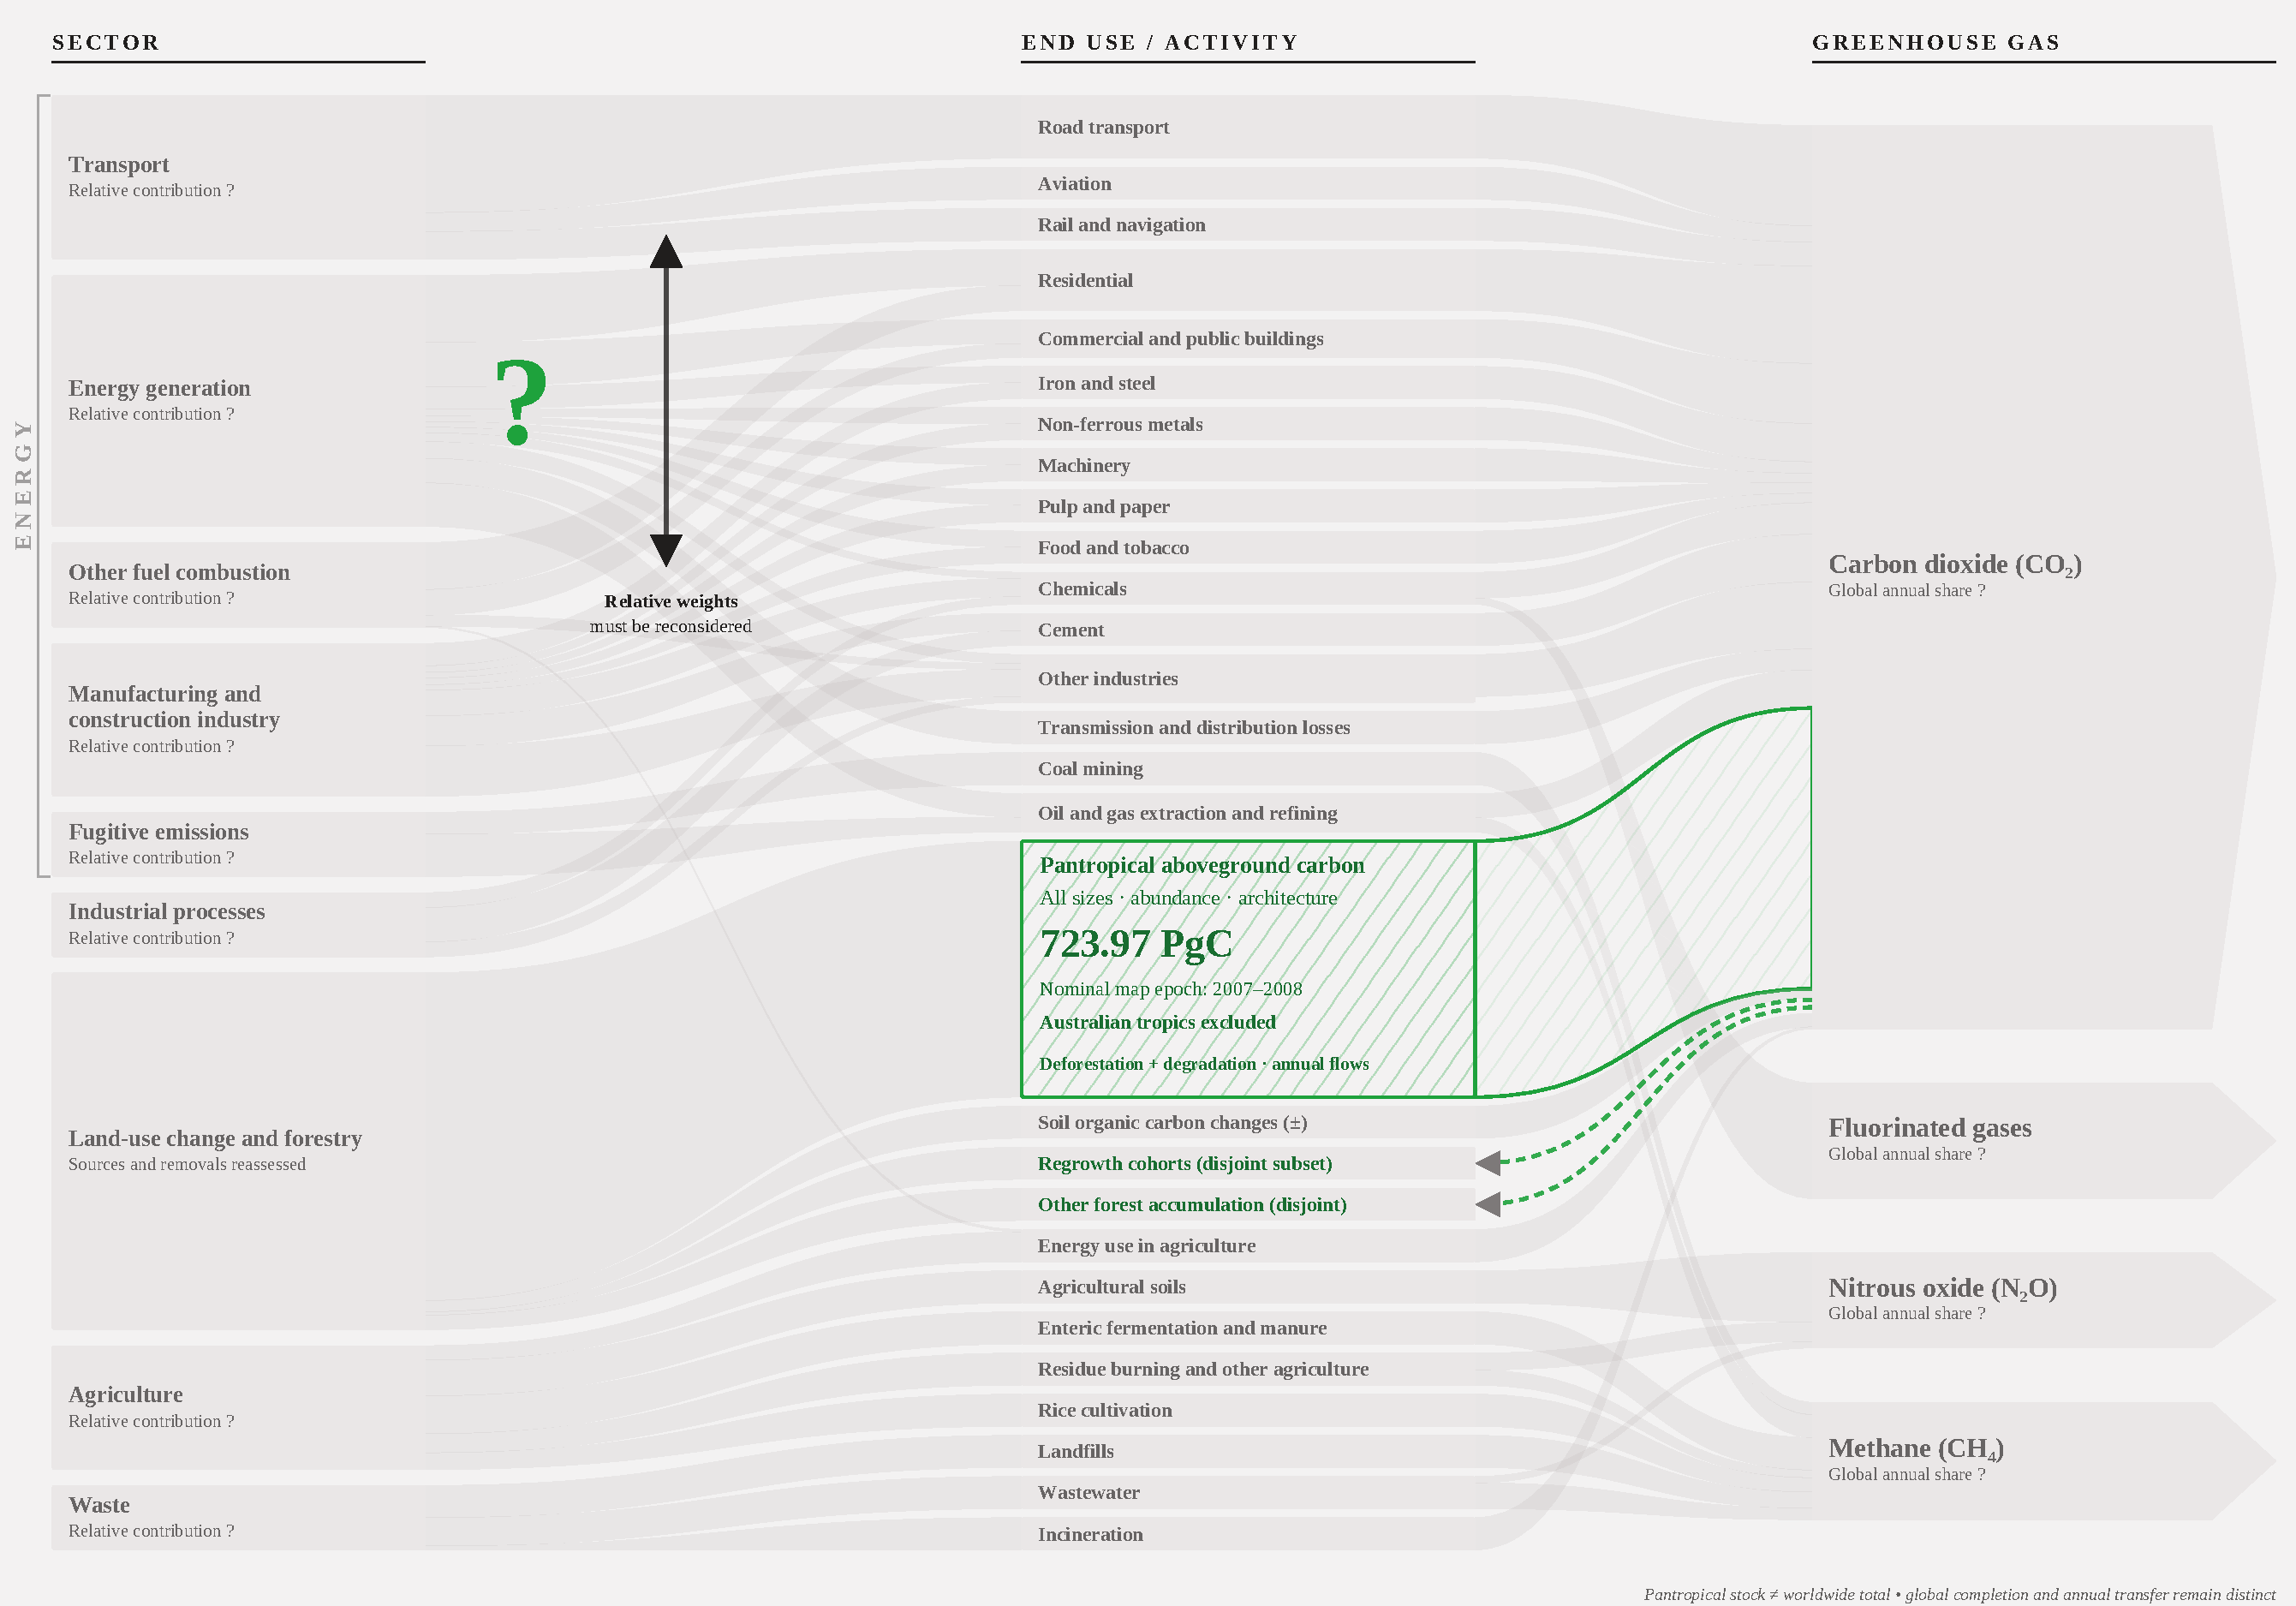
\includegraphics[width=365mm]{figures/figure2.pdf}\end{center}
\vspace{-2mm}
\fcolorbox{forestink}{papergray}{\parbox{.975\textwidth}{\small
\textbf{All sizes, not only the largest trees.} In the \textit{Acalypha}--\textit{Guazuma} community, the 10--30\,cm class contains 38.97\% of reported biomass in a community with total 147.8\,Mg\,ha$^{-1}$; 2.88 t divided by 30 stems gives a derived mean of \textbf{96 kg biomass per stem} (V\'asquez and Arellano, 2012, Table 170, p.~942). This older class distribution is allometry-based and illustrates abundance rather than class-5 density; the separate architectural records near 100\,kg illustrate that method's size coverage. Abundance, affected fractions and release histories govern population contribution.\\[1mm]
\textbf{Physical consequence and attribution.} A positive net source missing from an account leaves actual accumulation above the account's reconstruction unless other terms offset it. With total and removals held fixed, forest loss receives a larger share and can become the leading source if its corrected flux exceeds competing categories. Delayed release enters later years. Observed air can already contain emissions missed by an inventory; changing attribution does not itself establish an equally large measurement error in atmospheric concentration.}}\par
\vspace{2mm}
\fcolorbox{forestink}{papergray}{\parbox{.975\textwidth}{\vspace{1mm}
{\color{forestink}\textbf{SPATIAL COVERAGE: THE PANTROPICAL RESULT IS NOT A WORLDWIDE TOTAL}}\par\smallskip
\begin{tabularx}{\linewidth}{@{}p{.32\linewidth}p{.32\linewidth}X@{}}
\textbf{Mapped contribution: 723.97 PgC}\newline Aboveground carbon; Australian tropics excluded. & \textbf{Additional regional stock}\newline Australian tropics and extratropical vegetation require separate estimates. & \textbf{Worldwide completion}\newline Add compatible pools and dates; annual net exchange remains separate.\\
\end{tabularx}\par\smallskip
Nominal output-map reference: \textbf{2007--2008} (preprint p.~23). Baccini's \textbf{2012} publication describes a 2007--2008 map; Simard's height predictor uses 2005 GLAS data. Forest-only totals require a common forest mask.\par\medskip
{\color{forestink}\textbf{HISTORICAL 2010 ILLUSTRATION --- NOT A 2025 EMISSIONS ESTIMATE}}\par\smallskip
\textbf{Fixed total: 26.16--32.61\%. Other contributions retained: 22.58--26.66\%.} Both impose the stock multiplier on Ecofys's combined land-use category. The published 26.15--32.60\% endpoints are reproduced by truncation; alternative hidden precision is possible. Appendix B gives the source, assumptions and full calculation.\vspace{1mm}}}\par
\vspace{3mm}
\begin{minipage}{\textwidth}
\captionof{figure}{\textbf{Pantropical architectural measurement and worldwide annual attribution.} The green branch identifies 723.97 PgC as the mapped pantropical aboveground-carbon estimate, explicitly excluding the Australian tropics (Arellano-P. and Rangel-Ch., 2016, pp.~23--24). Its 2007--2008 nominal map epoch differs from publication and predictor-acquisition dates (Baccini et al., 2012; Simard et al., 2011). Global coverage additionally requires omitted tropical and extratropical vegetation on matched pool, mask and date definitions. Hatching denotes unresolved annual transfer, not rejection of the stock; graphical areas are schematic. The organization adapts the WRI/Ecofys source--activity--gas convention. Regrowth and other accumulation are disjoint conceptual subsets, not extra EDGAR subtotals. Muted sectors, the question mark and opposing arrows express a larger source total and reconstructed atmospheric burden under fixed other terms, a larger forest-loss attribution within a retained account, or joint reassessment. All stem sizes and partial degradation are included; no source ranking is inferred from graphical width. The historical inset is conditional 2010 arithmetic, not a measured 2025 allocation. Figure 3 states the independent structural protocol and its explicit comparison gap for class 5. Sections 2--3 specify measurement evidence; Sections 5--7 give annual-transfer conditions.}
\end{minipage}


\clearpage
{\large\bfseries\color{sourceblue} INDEPENDENT STAND-MEASUREMENT PROTOCOL}\hfill {Class 5: a two-sided calibration test}\par
\vspace{2mm}\hrule\vspace{1mm}
\begin{center}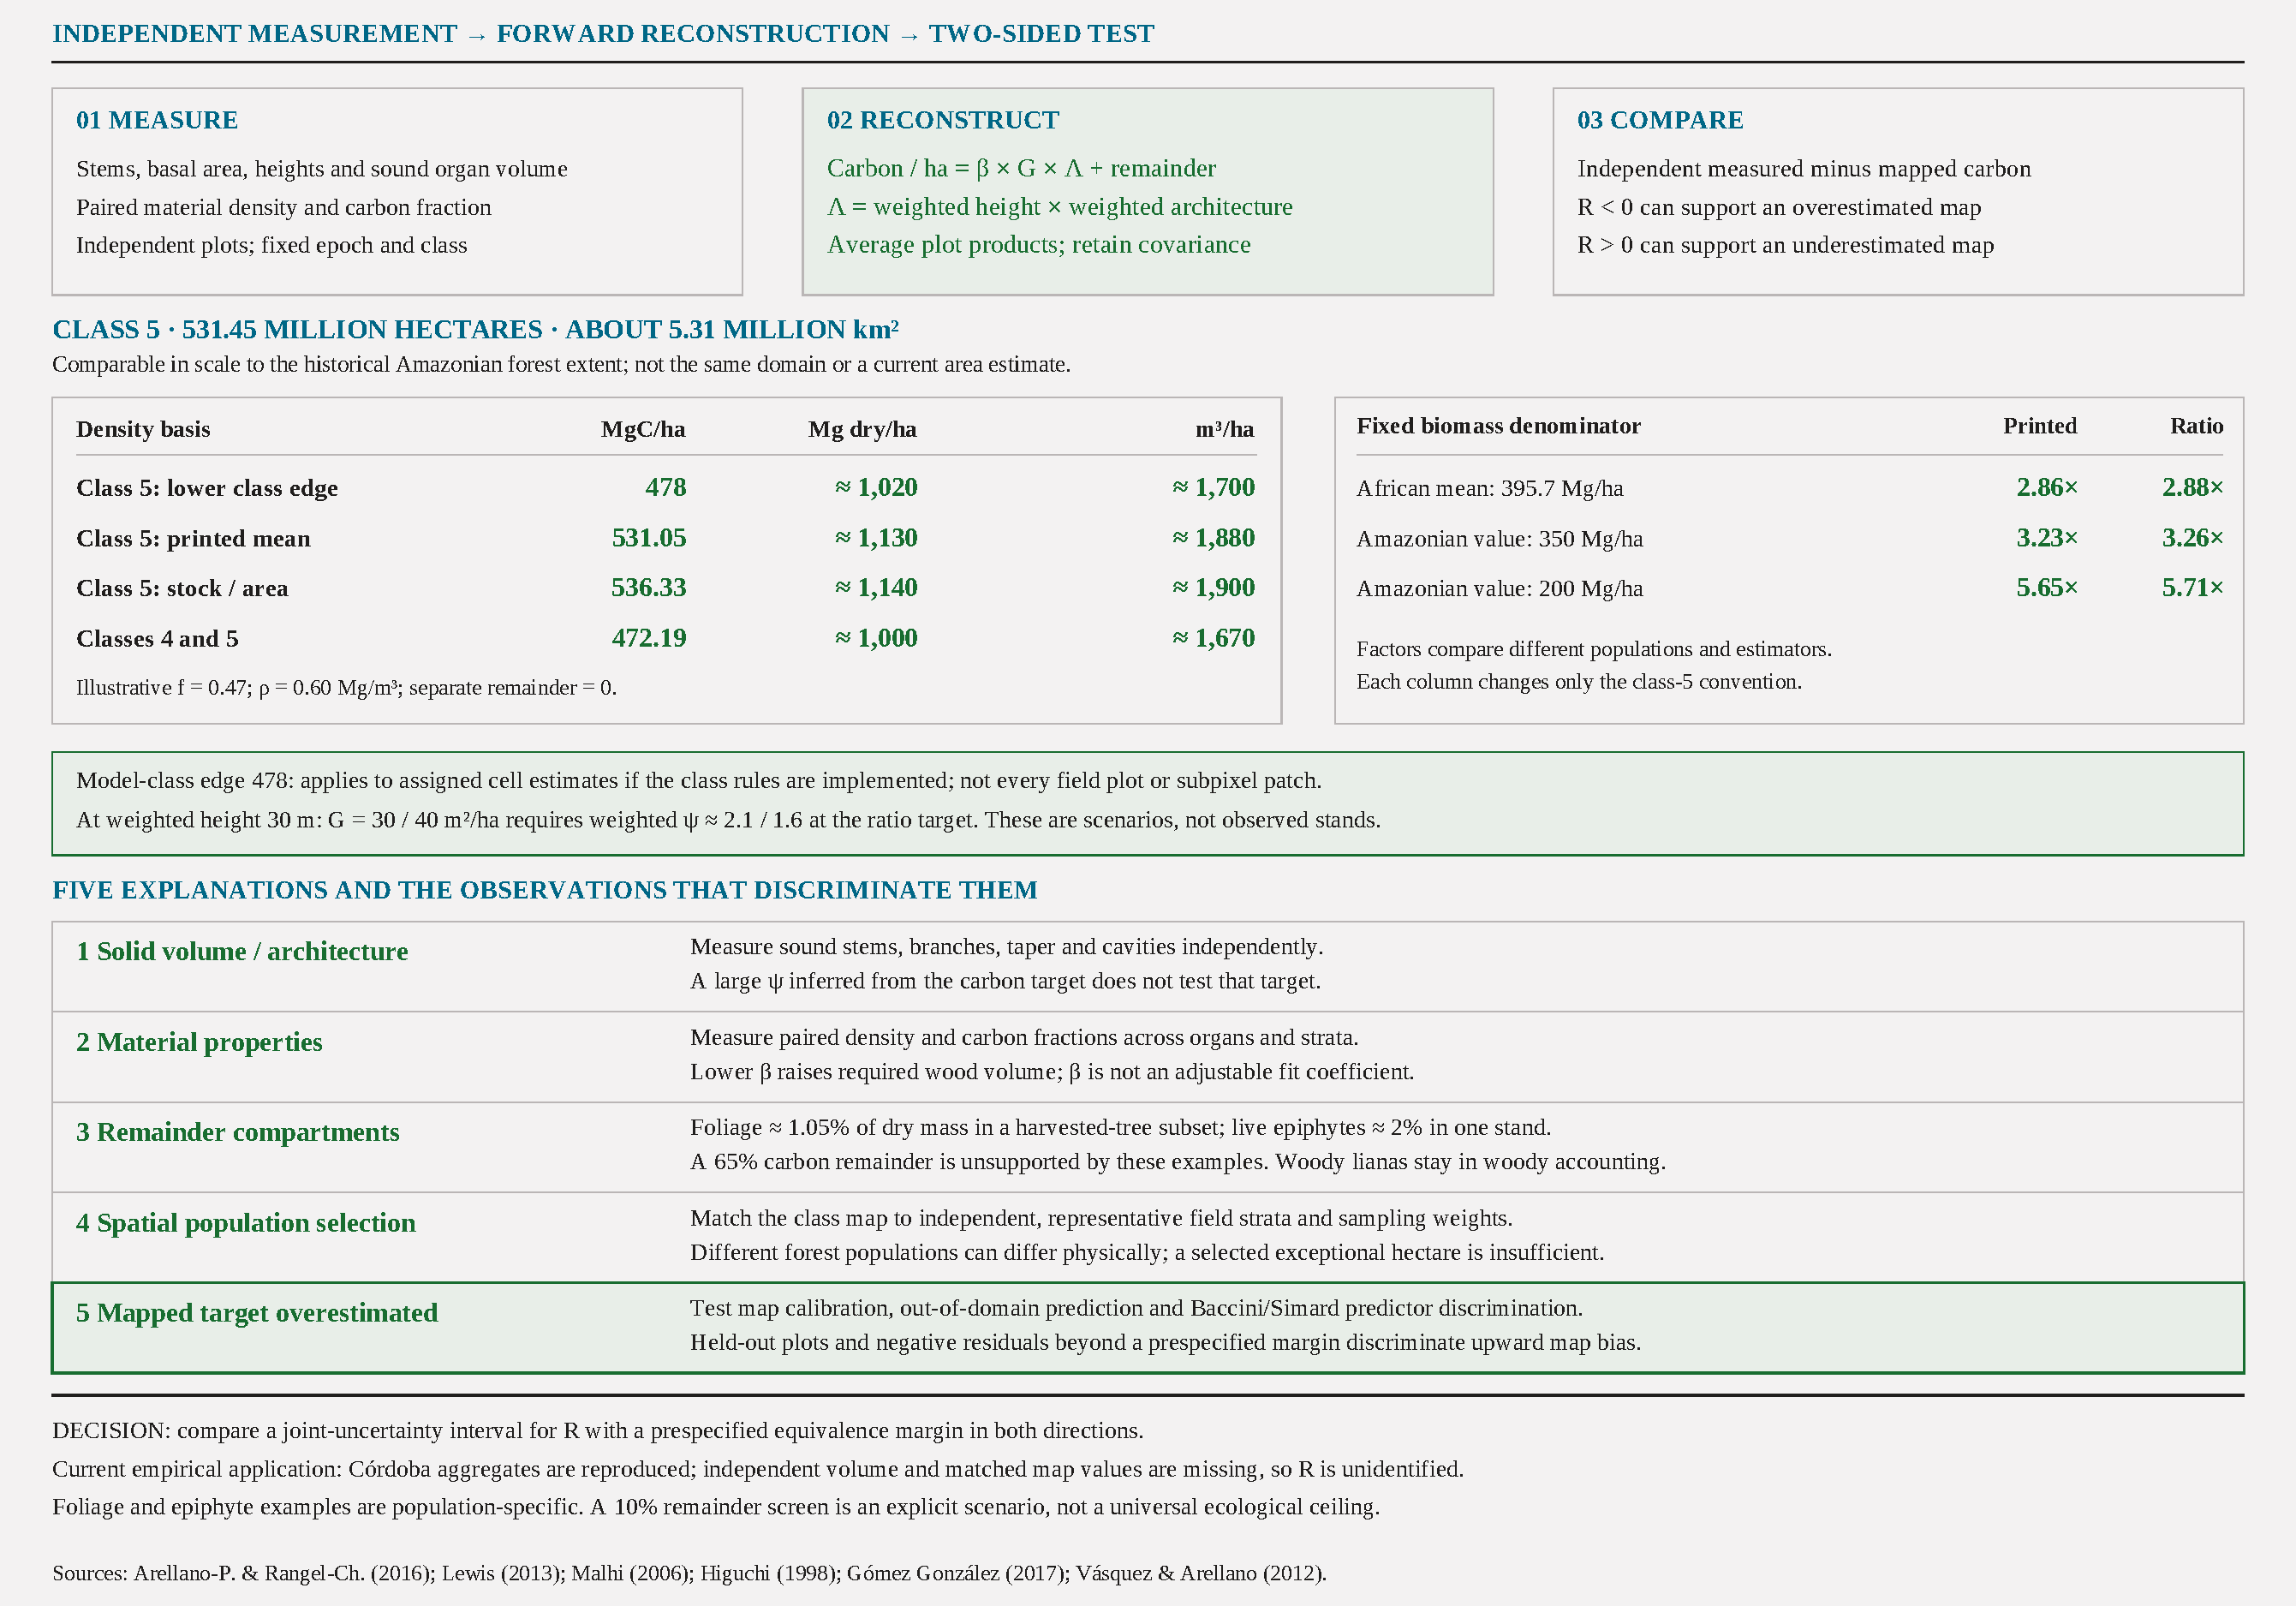
\includegraphics[width=390mm]{figures/figure3.pdf}\end{center}
\vspace{-2mm}
\fcolorbox{forestink}{papergray}{\parbox{.975\textwidth}{\small
\textbf{The target itself is tested.} Independent measured-minus-mapped residuals, with joint uncertainty and a prespecified margin, can support either an underestimated or an overestimated map. Geometry, material properties, remainder pools and spatial selection are evaluated alongside predictor discrimination, extrapolation and calibration bias. Foliage and ordinary live epiphytes are evidence-limited explanations, not unconstrained residuals; liana stems are woody. No class-5 empirical carbon residual has been recovered.}}\par
\vspace{3mm}
\begin{minipage}{\textwidth}
\captionof{figure}{\textbf{Five explanations of the class-5 discrepancy and their discriminating measurements.} The published class has a lower edge of 478 MgC ha$^{-1}$, a printed mean of 531.05 and a stock--area ratio of 536.33 (Arellano-P. and Rangel-Ch., 2016, Table 3). Conditional requirements assume carbon fraction 0.47, basic density 0.60 Mg m$^{-3}$ and zero separate remainder; public values are rounded, while computational precision is retained in the archive. The class edge applies to mapped-cell estimates if the classification implements that interval; it is not an observed lower bound on every hectare. The two comparison-factor columns change only the class-5 convention against fixed Lewis (2013) or Malhi (2006) biomass values. The dimensionless architecture ratio uses basal-area--height weights and sound woody volume. Higuchi et al. (1998), Table 3(b), gives a 1.05\% dry-leaf fraction as a ratio of sample totals in 38 harvested trees, distinct from the mean fresh-weight percentage. G\'omez Gonz\'alez et al. (2017) separates living epiphytes from dead organic matter and extrapolates sampled masses to one stand. Neither provides a universal remainder ceiling or a class-5 survey. The empirical C\'ordoba aggregate audit (V\'asquez and Arellano, 2012) records available observations and the missing inputs needed for a mapped-carbon residual. Approximately 5.31 million km$^2$ of class area is comparable only in scale to the historical 5.3 million km$^2$ Amazonian forest extent in Fauset et al. (2015). Original vector design and calculations: Henry Arellano-Pe\~na.}
\end{minipage}
\end{document}
